% Preamble
\documentclass[a4paper,12pt]{article}

\usepackage[osf]{mathpazo} % palatino
\usepackage{ms}            % load the template
%\usepackage[round]{natbib} % author-year citations
\usepackage[superscript,biblabel]{cite} % for superscript citations
\usepackage{graphicx}
\usepackage{parskip} 
\usepackage{caption}
\usepackage{subcaption}
\usepackage{textcomp} % for parts per mille symbol     
\pagenumbering{arabic}    
\linespread{1.66}


% -------------------------------------------------------------------------------------------------------
% some custom commands

% Add support for highlighting
\usepackage{color}
\newcommand{\hilight}[1]{\colorbox{yellow}{#1}}

% -------------------------------------------------------------------------------------------------------

% Title page information
\title{Reconstructing the last known movements of one of Nature's giants}
% 90 characters max

\author{
  Clive N. Trueman$^{1}$, Andrew L. Jackson$^{2}$, Katharyn S. Chadwick$^{1}$,\\ 
  Ellen J. Coombs$^{3,4}$, Sarah Magozzi$^{1,5}$, Richard C. Sabin$^{3}$ \\
  and Natalie Cooper$^{3*}$
}
\date{}
\affiliation{\noindent{\footnotesize
  $^1$ Ocean and Earth Science, University of Southampton Waterfront Campus, Southampton, SO14 3ZH, UK.\\
  $^2$ School of Natural Sciences, Trinity College Dublin, Dublin 2, Ireland.\\
  $^3$ Department of Life Sciences, Natural History Museum London, Cromwell Road, London, SW7 5BD, UK.\\ 
  $^4$ Department of Earth Sciences, University College London, Gower Street, London, WC1E 6BT, UK.\\
  $^5$ Department of Geology and Geophysics, University of Utah, Salt Lake City, UT 84112-0102, USA.\\
}}

\vfill

%\runninghead{}
%\keywords{}
%}

% End of preamble

\begin{document}
\modulolinenumbers[1]   % Line numbering on every line

\mstitlepage

\parindent = 1.5em
\addtolength{\parskip}{.9em}
% Abstract 200 -300 words max
% \section{Abstract}
% general topic intro - 1 sentence
% intro to field - 2 sentences
% what we find/show - 1 sentence
% implications - 2-3 sentences. Results in context, how has the paper moved the field forward

\raggedright

\section{Abstract}
Understanding animal movements is crucial for effective conservation, especially as species ranges shift due to climate change\cite{runge2014conserving,robinson2009travelling}. 
Animal tissues housed in museum collections provide biochemical records of behaviour that can be used to reconstruct individual-level movements over long timescales and under historical climatic and ecological conditions\cite{newsome2010using}, but interpreting these records can be challenging. 
Here we combine stable isotope analyses of baleen with novel agent-based simulation models, to reconstruct seven years of movements of an iconic female blue whale (\textit{Balaenoptera musculus}) that stranded off Ireland in 1891 and is now on display at the Natural History Museum, London. 
We provide the longest continuous record of movement for an individual blue whale in the north Atlantic. 
We show that the whale spent at least two years resident in sub-tropical waters as a juvenile, before commencing annual latitudinal migrations consistent with patterns of movements of blue whales in the northeast Atlantic inferred from observations, tagging and historic whaling data. 
The isotopic record is consistent with observations of opportunistic feeding throughout the year in blue whales, and suggests pregnancy and calf-rearing in the year before death.
Historic tissue collections can provide unique insight into individual-level movement behaviours associated with changing climate, ecological conditions and anthropogenic pressures, and reveal aspects of life history. 
Combining biochemical tracers with simulation modeling unlocks the information recorded in these irreplaceable archives.

\newpage
\section{Main text}
Migratory species pose a particular challenge for conservation practitioners because their effective conservation relies on protection at many, often distant, sites\cite{runge2014conserving}. 
Migratory species may also be particularly vulnerable to changes in climate or human use of the environment, as they are influenced by conditions in multiple locations across different parts of their life cycle\cite{robinson2009travelling}. 
Identifying threats to migratory species and developing effective conservation measures requires information on individual-level movements spanning multiple years, for both historical and present-day populations. 
Such data are scarce, especially for rare, wide-ranging and long-lived marine species\cite{ryan2013stable,hall2005stable,bailey2009behavioural}. 
 
The blue whale (\textit{Balaenoptera musculus}), the largest animal to have ever lived, is one such migratory marine species. 
Despite hunting for blue whales being banned for over 50 years, blue whales are still listed as Endangered on the IUCN Red List\cite{reilly2008balaenoptera}.
In the northeast Atlantic, blue whales appear to form a separate population, with little evidence for exchange between northeast and northwest Atlantic populations\cite{pike2009note}.  
The northeast Atlantic population of blue whales was the first large whale population to be systematically hunted with explosive harpoons, and while the population was probably relatively small before hunting, now fewer than 1000 individuals are estimated to be in the northeast Atlantic in summer, mainly distributed around Iceland\cite{pike2009note}.
Following movements of individual blue whales is extremely challenging due to their scarcity and oceanic habit.
Similar to other large balaenopterid whales, blue whales in the northeast Atlantic are generally assumed to conduct annual migrations between high and low latitudes. 
A combination of historic whaling data, observations, satellite tracks and acoustic monitoring suggest that blue whales in the northeast Atlantic track regions of high production throughout the year, with at least some whales wintering in the upwelling systems between Mauritania and the Cape Verde Islands\cite{baines2014upwellings}.
Northward migration in the spring may occur along mid-Atlantic corridors with peak sightings in the Azores around April-May. Summer feeding appears to occur in northerly latitudes around Iceland, and historically in the Norwegian and Barents Seas\cite{pike2009note}.
Blue whales are frequently detected in waters to the west of the UK, with peak acoustic detections occurring between November and December, in southward-migrating animals\cite{reeves2004historical,baines2017autumn,charif2009acoustic,visser2011timing}.
While direct tagging methods are adding vital behavioural data to our understanding of whale movements\cite{borger15,mcdonald2006biogeographic,bailey2009behavioural,mate2007evolution,silva2013north}, they are often expensive, limited to short-term studies\cite{bailey2009behavioural,best2015tag,mate2007evolution}, and may influence whale behaviour\cite{walker2012review}.
Conservation efforts are consequently hampered by the lack of detailed data on the distribution, behaviour and ecology of blue whales, particularly during the winter and for the juvenile phase of life. 
An alternative technique for investigating whale movements retrospectively is to use intrinsic biochemical information such as stable isotopes\cite{west2006stable,busquets2017estimating,hobson2008tracking}. 
The stable isotope composition of animal tissues reflects the isotopic composition of diet at the time and place of ingestion, integrated over the timescale of tissue growth. 
Stable isotope data therefore provide information on diet and location (i.e. `trophic geography'\cite{bird2018global}), but incomplete knowledge of the spatio-temporal distribution of the isotopic composition of prey currently limits interpretation of measured values. 
Here we reconstruct movements of an historic whale by comparing isotopic compositions of samples from museum collections, rich archives of behavioural information\cite{lister2011natural}, to spatially referenced models of isotopic variation in diet across the northeast Atlantic \cite{hobson1999tracing,hobson2008tracking,eisenmann2016isotopic}. 

Mysticete (baleen) whales are characterized by the development of baleen plates, keratinous structures in the upper jaw used to filter food items from seawater. 
Baleen is ideal for stable isotope studies because keratin grows continuously through an individual's life, and once laid down it is metabolically inert\cite{best1996stable}. 
Baleen plates therefore offer a continuous isotopic record of behavior reflecting multiple years of life of an iindividual whale, although as baleen is worn away at the tips over time, an individual's entire lifespan is rarely recorded. 
Baleen stable isotope records have a long history of use as biochemical markers to infer movement patterns in whales\cite{ryan2013stable,best1996stable,hobson1998stable,hobson2008tracking}, but have yet to be applied to blue whales from the north Atlantic population. 
Here we apply this method to baleen from the Natural History Museum London's (NHM) blue whale ``Hope''. 
Hope is female, and estimated to be a young adult c.15 years at death, suggesting that her baleen may yield information about juvenile behaviours in north Atlantic blue whales around the peak of industrial whaling.
 
Blue whales feed mainly on krill (Euphausiacea), small crustaceans that feed on phytoplankton \cite{handbook}.
Thus the stable isotope compositions of keratin at a given point in the baleen will reflect the stable isotope compositions of the krill it was feeding on.
We sampled keratin from the blue whale's baleen plate at 1cm intervals perpendicular to the direction of growth, resulting in 97 discrete samples of baleen.
We then used continuous-flow isotope ratio mass spectrometry to determine the isotopic compositions of carbon and nitrogen in the keratin.
These isotopes are expressed as $\delta^{13}$C and $\delta^{15}$N values, i.e. relative to a standard and as ratios of the rare ($^{13}$C, $^{15}$N) to common ($^{12}$C, $^{14}$N) isotope\cite{west2006stable}.
Carbon and nitrogen isotopes are commonly reported together as they provide complementary information; both isotopes provide information on the geographical locations of an individual, but nitrogen isotopes are more strongly fractionated during protein metabolism and thus contain additional trophic and physiological information\cite{west2006stable}.

Throughout the record, $\delta^{15}$N values record regular cyclical fluctuations, with a mean spacing of 13.5cm, assumed to represent annual periodicity (see Supplementary Methods; Supplementary Figures S1 and S2). 
Therefore, given the date of stranding (25th March 1891), and estimated baleen growth rates of 13.5cm $y^{-1}$, we reconstructed a timeline for $\delta^{13}$C and $\delta^{15}$N fluctuations in the baleen over seven full years of the whale's life (early 1884 - spring 1891). 
The $\delta^{13}$C and $\delta^{15}$N profiles show two distinct phases in the whale's behaviour. 
In behavioural phase one (from the start of the record in early 1884 to spring 1886), we find relatively stable, elevated $\delta^{13}$C values, and relatively low $\delta^{15}$N values (Figure \ref{fig1}; Supplementary Figures S1 and S2). 
In behavioural phase two (summer 1886 to spring 1890) $\delta^{15}$N values are relatively high and $\delta^{13}$C values are relatively low with coincident cyclical fluctuations in both $\delta^{13}$C and $\delta^{15}$N values. 
In the last year of life the cyclical pattern is disrupted, with constant low $\delta^{13}$C values for approximately six months in the first half of 1890, before a rapid switch to relatively high $\delta^{13}$C values in the second half of 1891. 
The final three months of the record show a progressive fall in $\delta^{13}$C values (Figure \ref{fig1}; Supplementary Figures S1 and S2).

% figure 1
\begin{figure}
  \centering
  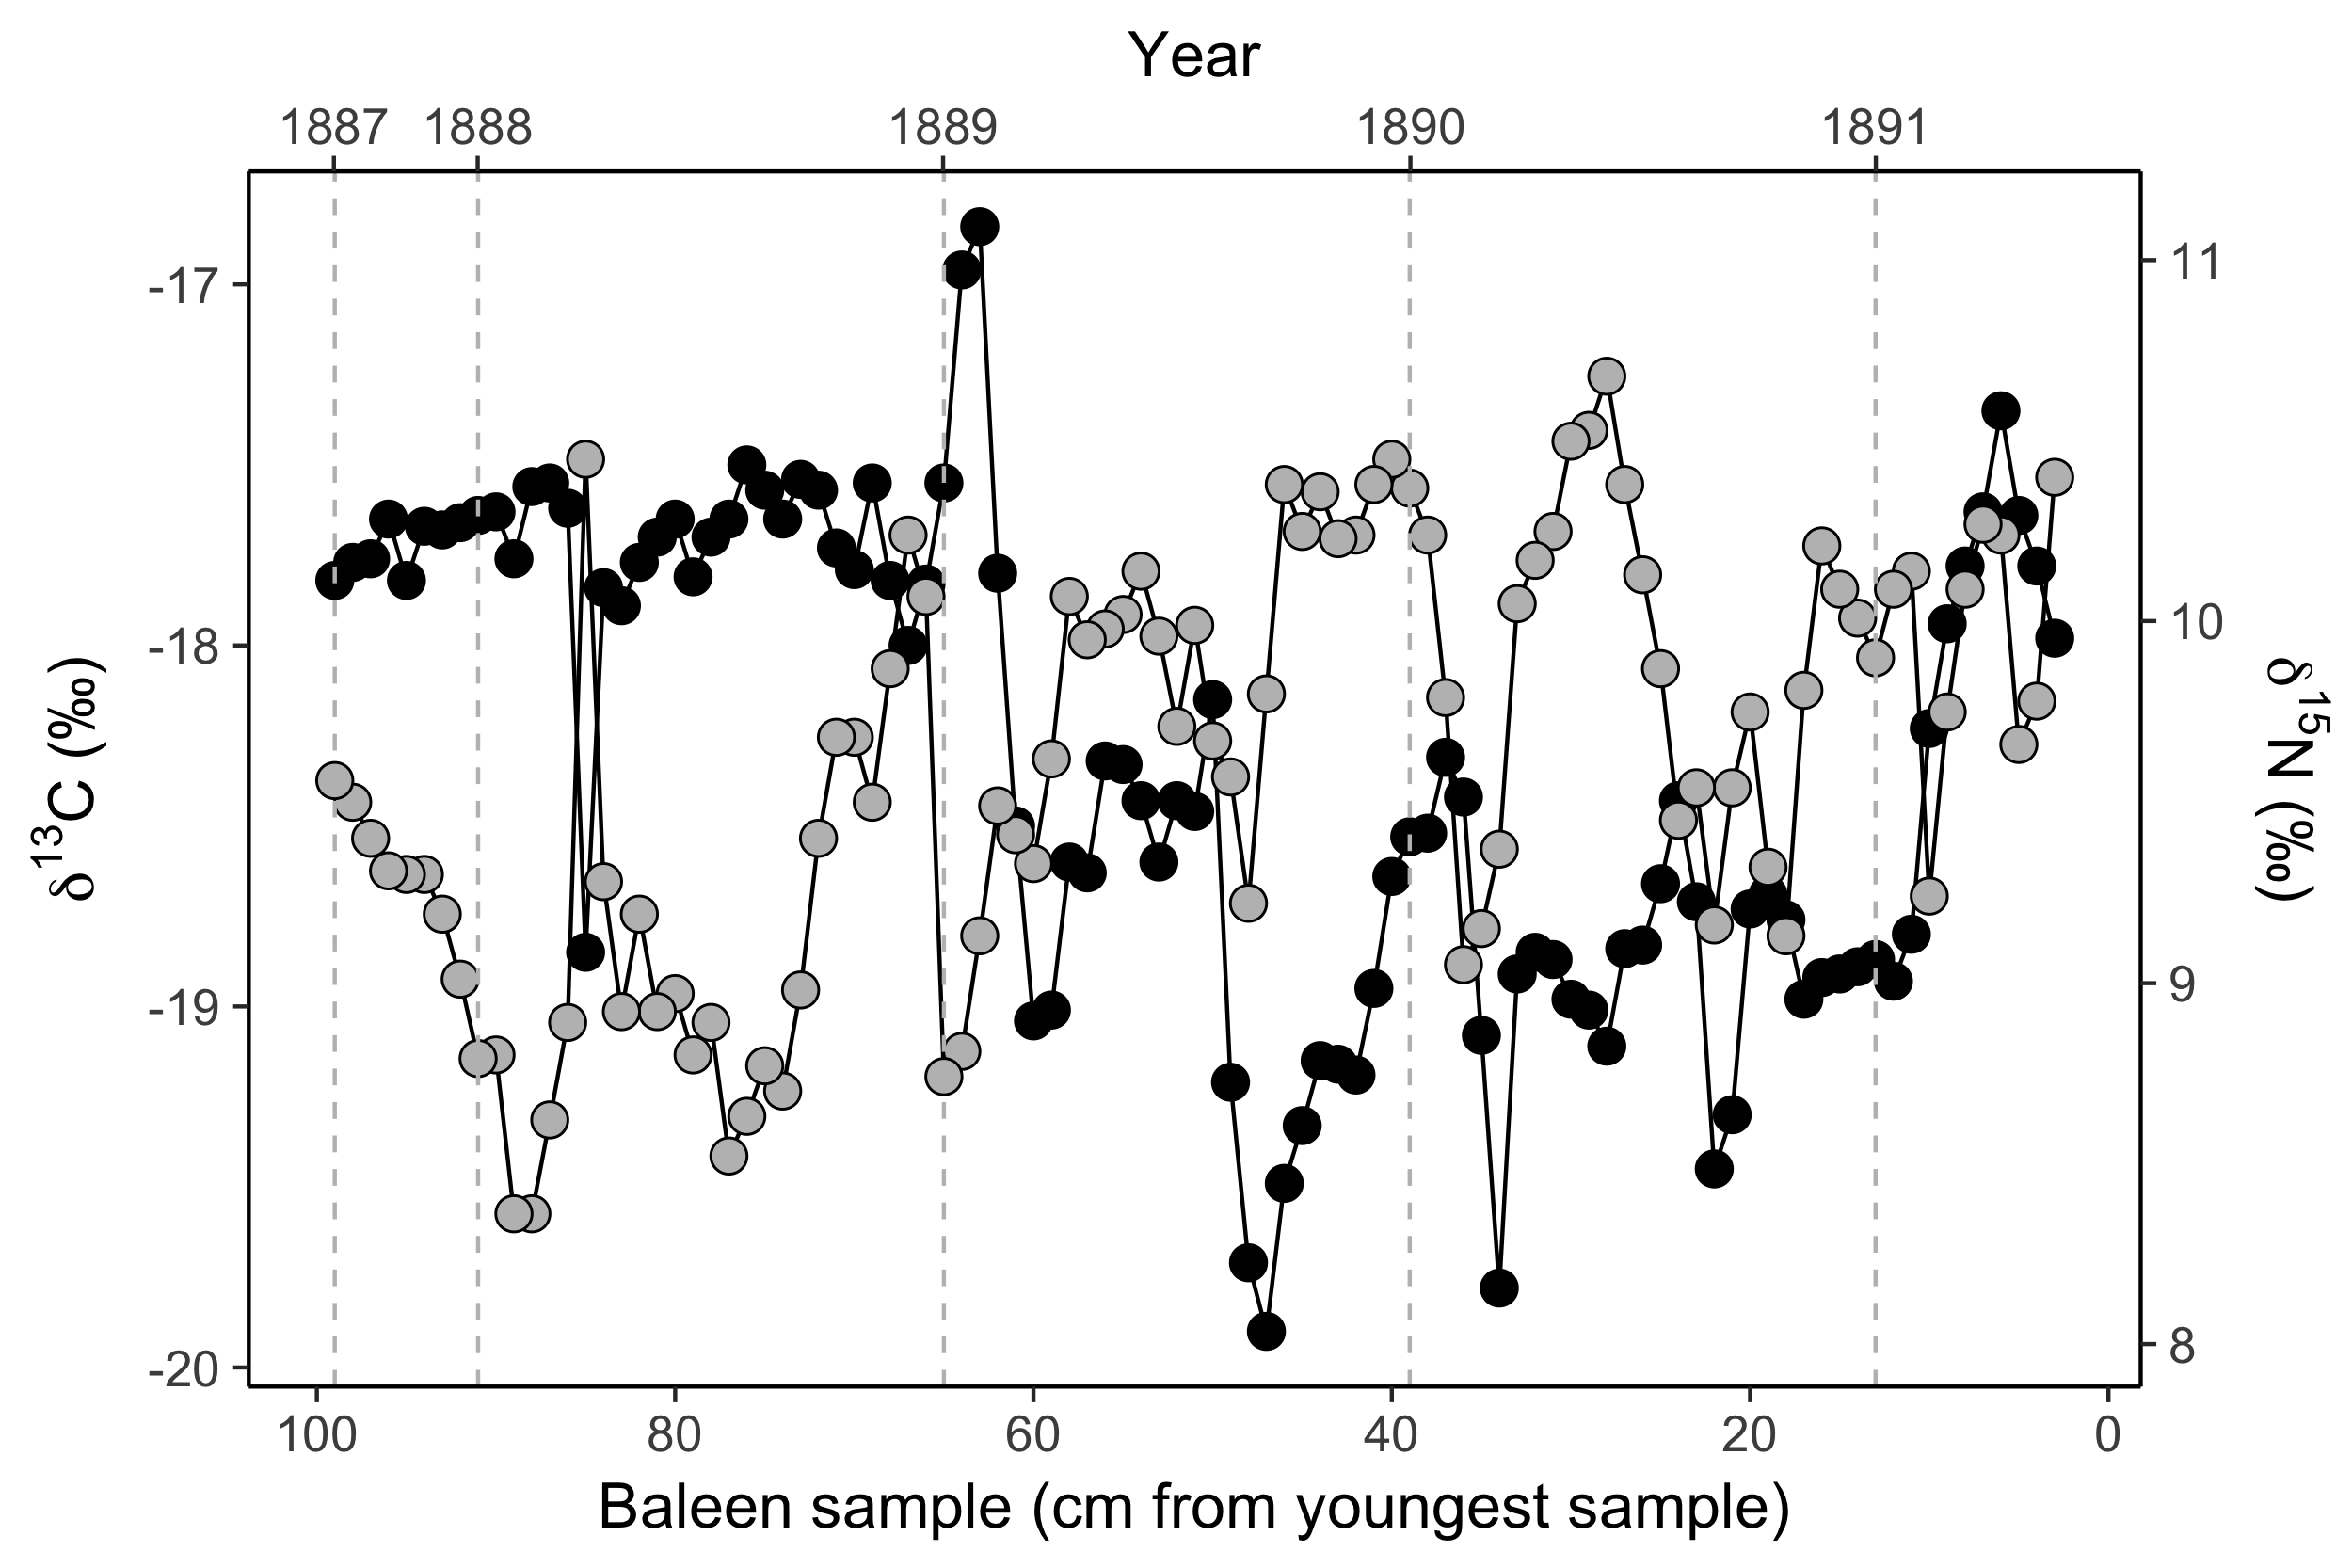
\includegraphics[width = \linewidth]{figures/Figure-1-raw-dC-dN-data.png}
  \caption{Variation in stable isotope values in the NHM blue whale, expressed as $\delta^{13}$C (black circles, left y-axis) and $\delta^{15}$N (grey circles, right y-axis). Samples were taken longitudinally through the baleen plate (n = 97 samples from a single baleen plate for both isotopes). There is strong annual periodicity and cross-correlation (Supplementary Figures S1 and S2) in both isotopes. The approximate relationship to years assuming a growth rate of 13.5cm y$^{-1}$ is shown on the upper x-axis, and year boundaries are indicated by vertical dotted grey lines.}
  \label{fig1}
\end{figure}

Relating the isotopic compositions of animal tissues to likely locations is complicated by a lack of knowledge of spatio-temporal variations in the isotopic composition of diet\cite{west2006stable,mcmahon2015millennial}.
We develop a new approach to address this problem using temporally dynamic models of $\delta^{13}$C values in the global ocean\cite{magozzi2017using} (Supplementary Figure S3), coupled to an agent-based model of whale movements (see Supplementary Methods; Supplementary Table S1; Supplementary Figure S5).  
We use our coupled model to simulate time series of $\delta^{13}$C values expected under differing movement behaviours and in differing parts of the known geographic range of north Atlantic blue whales. 
We then compare simulated profiles (Figures \ref{fig2}, \ref{fig3} and Supplementary Figure S4) to the measured isotopic profile of the blue whale's baleen (Figure \ref{fig1}) to identify the most likely movement history. 
Blue whales are commonly assumed to feed mainly in summer in productive, high latitude regions and rely largely on stored lipid reserves to meet metabolic demands in lower latitudes in winter. 
However, in winter blue whales in the northeast Atlantic are associated with upwellings\cite{baines2017autumn}, while northward migrations in spring coincide with the onset and development of phytoplankton blooms\cite{silva2013north,visser2011timing,busquets2017estimating}, strongly implying feeding throughout the year. 
We therefore assume opportunistic ingestion of protein throughout the year. 

% figure 2{}
\begin{figure}
 \centering
 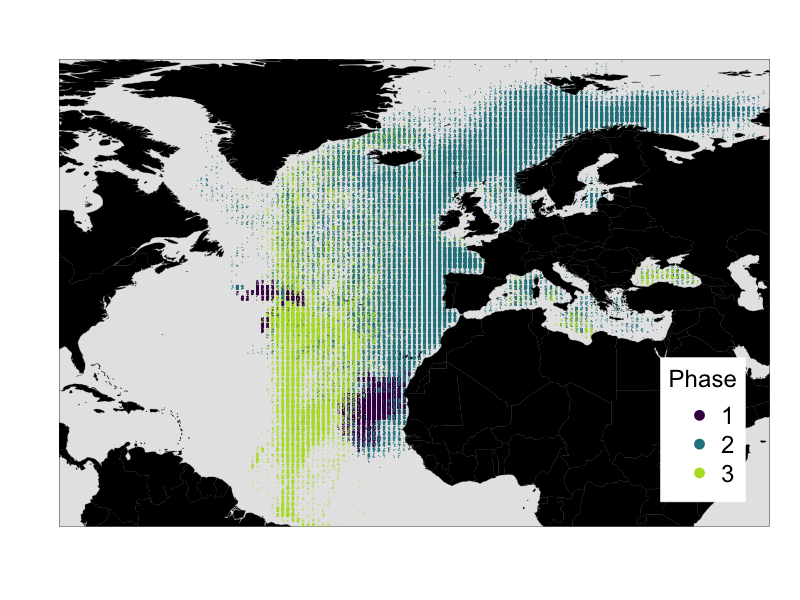
\includegraphics[width = \linewidth]{figures/Figure-2-points.png}
  \caption{Simulated locations of the whale taken from the top 10\% best fitting migratory movement models. 
  Colours reflect the behavioural phase. 
  Phase one is early 1884 to spring 1886, phase two is summer 1886 to spring 1890, and phase three is spring 1890 to spring 1891.}
  \label{fig2}
\end{figure}

% figure 3
\begin{figure}
 \centering
  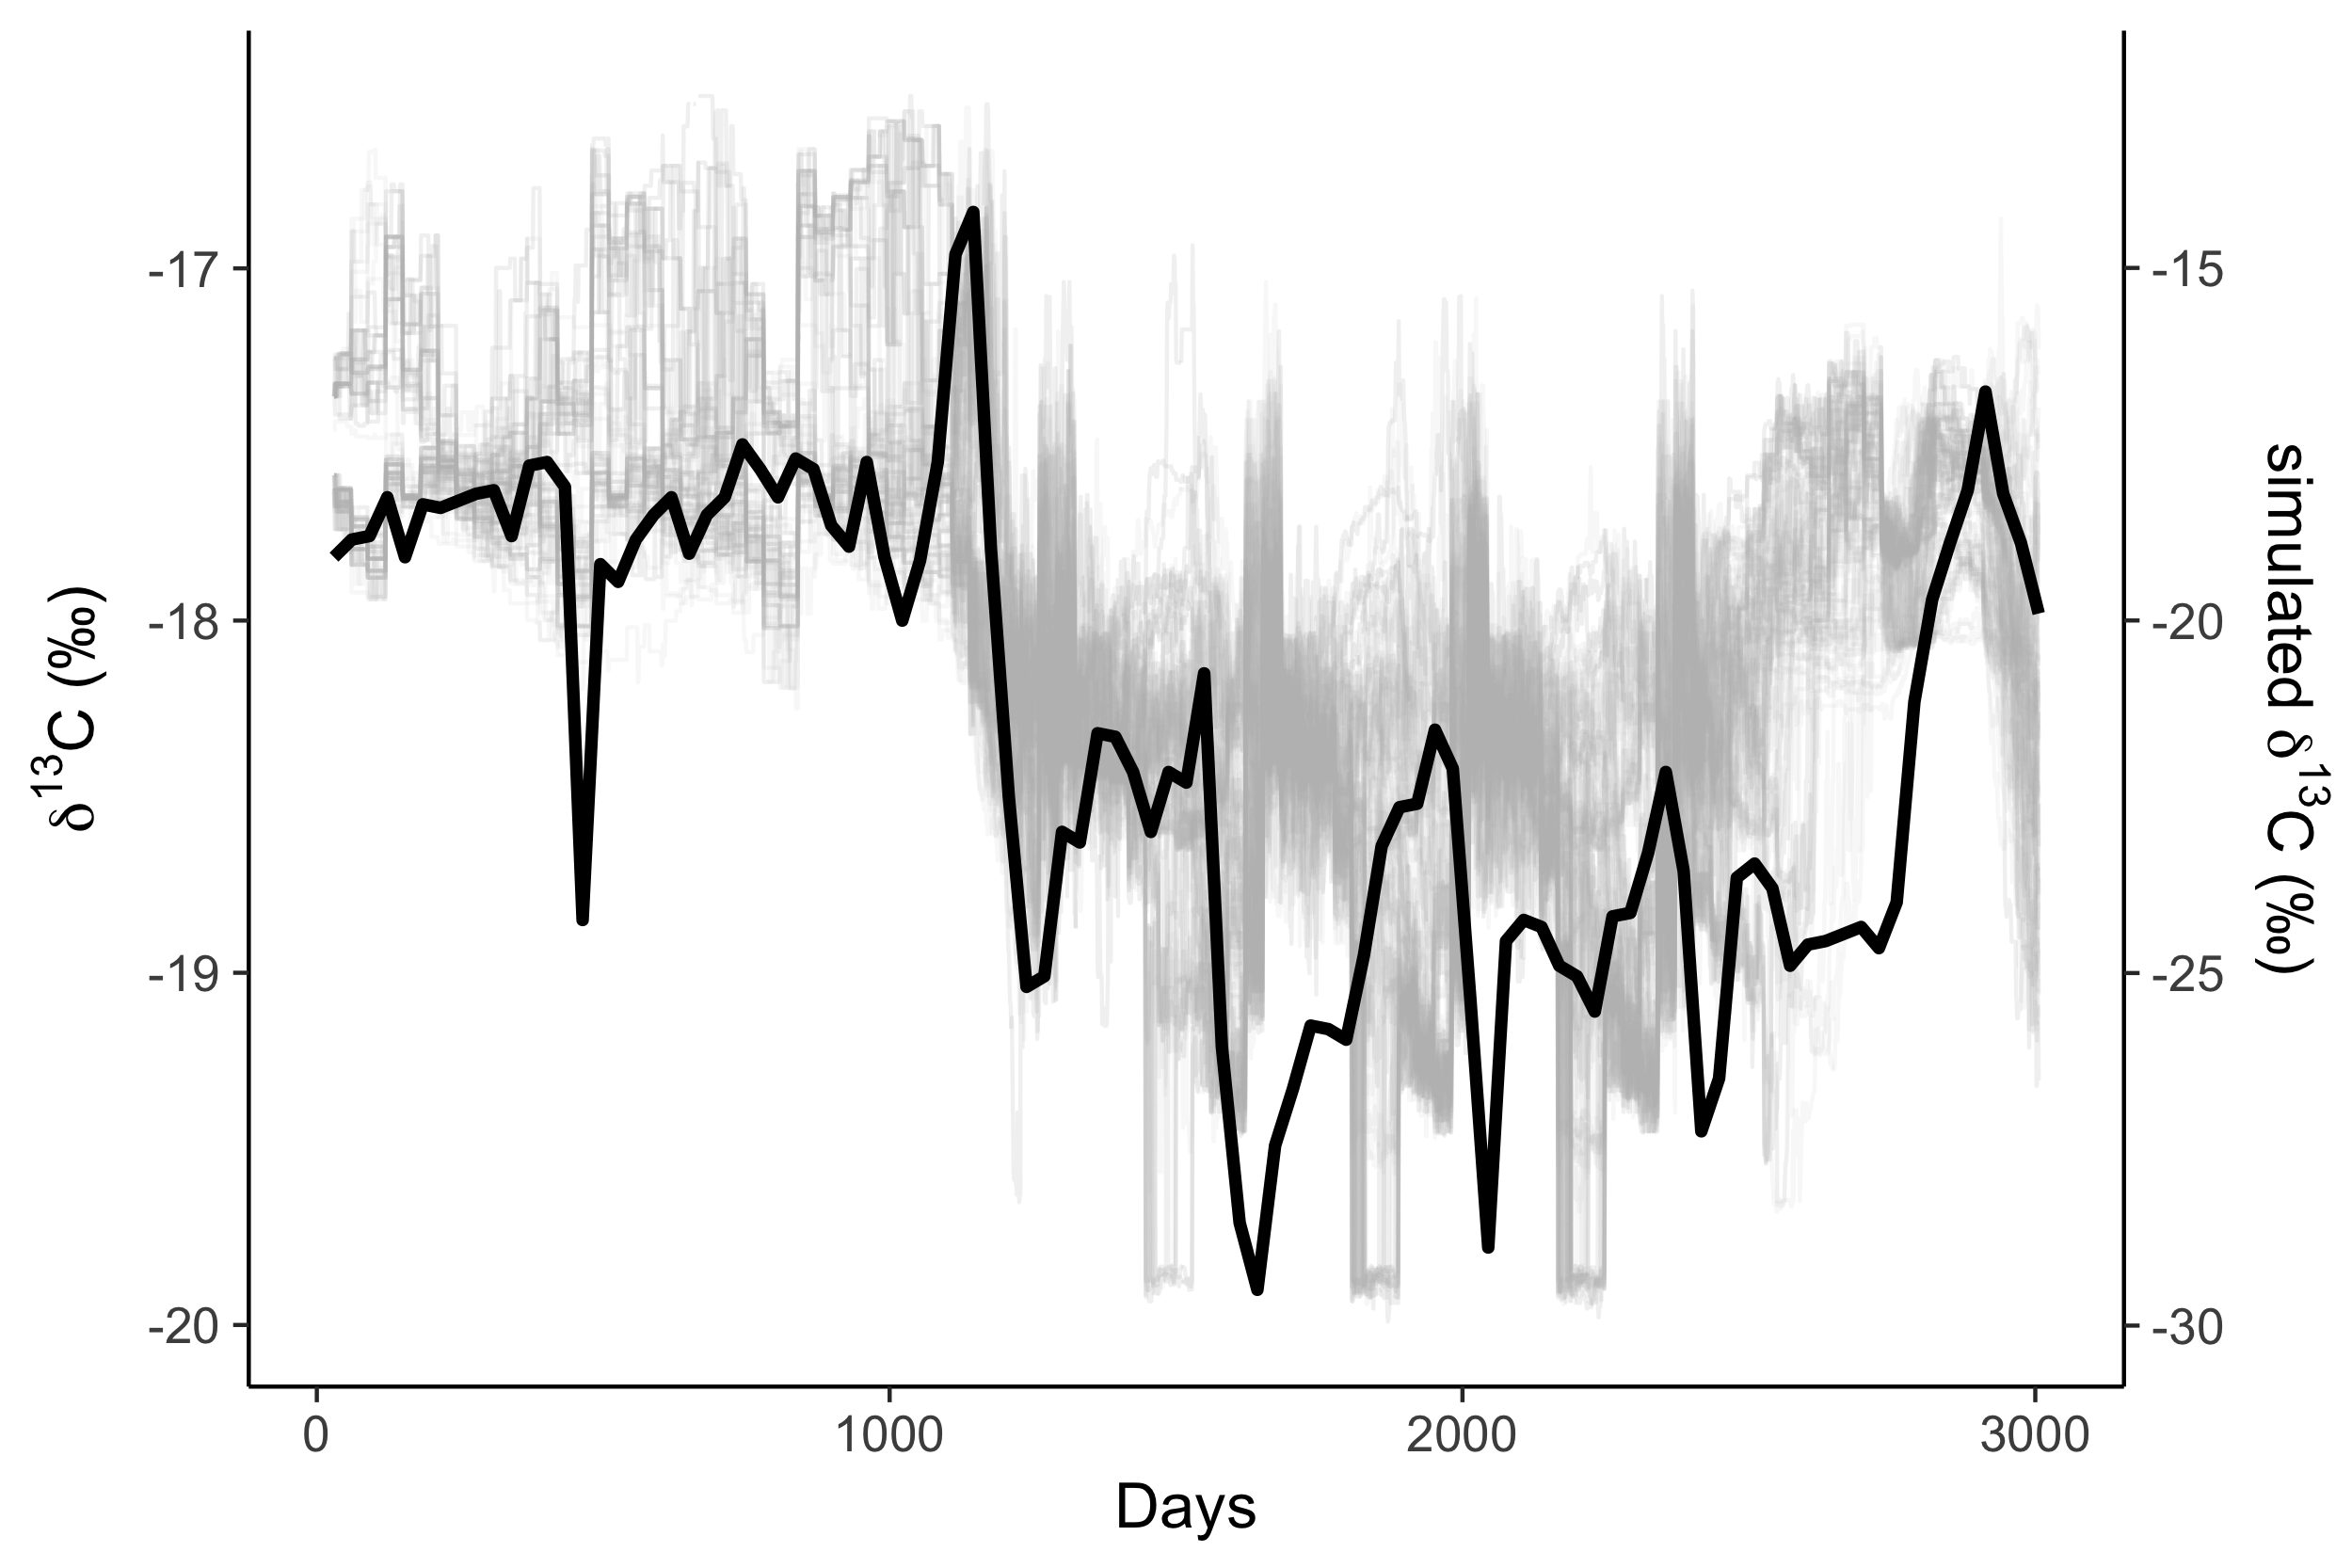
\includegraphics[width = \linewidth]{figures/Figure-3-blue-sims.png}
  \caption{Correlations among simulated $\delta^{13}$C from the top 10\% best fitting migratory movement models (grey lines, right hand y-axis) and $\delta^{13}$C from baleen (black line, left hand y-axis; see Figure \ref{fig1}). 
  Simulated $\delta^{13}$C values six month moving average values for the time series of simulated plankton $\delta^{13}$C values in that location, reflecting temporal integration of phytoplankton $\delta^{13}$C values within the food chain before ingestion by the whale as krill. 
  The end points of the simulations and empirical data have been aligned to coincide.
}
  \label{fig3}
\end{figure}
 
The relatively positive and seasonally-invariant $\delta^{13}$C values seen during behavioural phase one are only found in sub-tropical areas of the North Atlantic.  
Our simulations show high variance during this period (Figure \ref{fig3}), reflecting a range of possible locations for the whale, although areas around the Mauritanian coast and Cape Verde islands, a known current and historic winter feeding area for blue whales \cite{baines2014upwellings,reeves2004historical}, and potentially to the west of the Azores (Figure \ref{fig2}), most closely match the measured profile. 
The whale remained in relatively warm waters for at least two full years. 
Hope was estimated to be 15 years old when she died (based on vertebral epiphyseal fusion; R.Sabin \textit{pers.comm}), so was approximately 3-5 years old during this period.
During behavioural phase two, starting at an approximate age of 5-6 years, the observed low $\delta^{13}$C values imply foraging in colder, more northerly latitudes. 
The pronounced cyclical variations in $\delta^{13}$C values observed during behavioural phase two could reflect either the isotopic expression of the spring phytoplankton bloom in northern waters \cite{magozzi2017using}, latitudinal migrations, or a combination of both.  

We simulated 1200 individual movement patterns, then excluded simulations where the virtual whale stranded before reaching the 3019 days represented in the baleen.
With then compared the remaining 1049 simulations and the resulting simulated baleen $\delta^{13}$C records to the measured records with simple linear regressions. 
Simulated baleen $\delta^{13}$C profiles produce a good fit to measured profiles, the median $r^2$ value across 1049 simulated profiles was 0.49, and the maximum was 0.71 (Supplementary Figure S6).
The top 10\% best fitting simulated profiles are shown in Figure \ref{fig2}. 
Best fitting models predict juvenile residency in the Cape Verde region in behavioural phase one. 
Behavioural phase two is best simulated by seasonal migrations between summer foraging in northern areas in the Norwegian Sea/Barents Sea/Iceland region, and winter foraging in a broad region between the UK and more southerly, sub-tropical waters. 
Better fitting models in general were those predicting a greater latitudinal foraging range, and foraging in more northerly waters (Supplementary Figures S7 and S8).
Best-fit model distributions are largely consistent with our current understanding of blue whale distributions in the northeast Atlantic\cite{reeves2004historical,baines2014upwellings,baines2017autumn,reeves2004historical}, with perhaps greater importance of winter foraging in temperate regions (Figure \ref{fig4}).

% figure 4
\begin{figure}
 \centering
  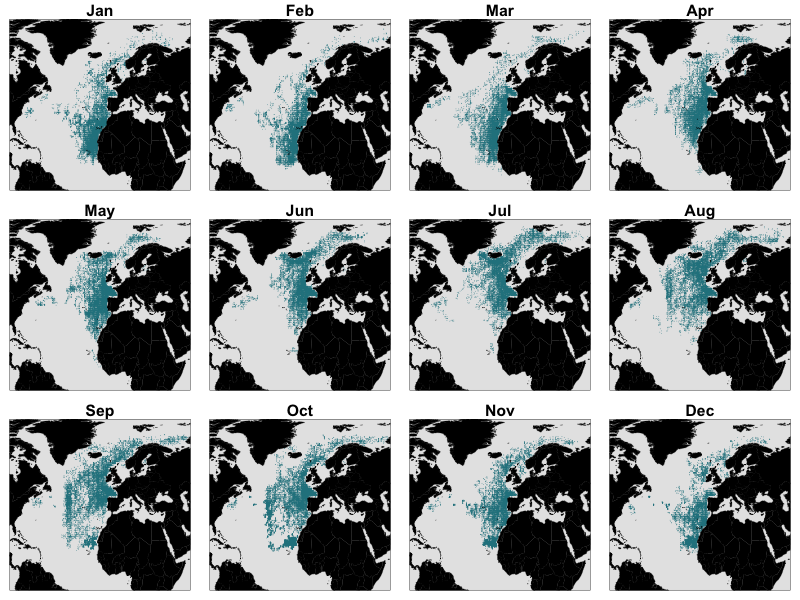
\includegraphics[width = \linewidth]{figures/Figure-4-monthly.png}
  \caption{Simulated locations by month taken from the top 10\% best fitting migratory movement models for behavioral phase two (summer 1886 to spring 1890) only.}
  \label{fig4}
\end{figure}

The isotopic record of the last 500 days of the whale's life are difficult to simulate. 
Beginning in the winter of 1889/1890, the observed $\delta^{13}$C values are relatively low, and remain constant for approximately six months, before increasing rapidly in the winter of 1890/1891. 
Low $\delta^{13}$C values are found in northern waters, but these regions also show large temporal fluctuations in $\delta^{13}$Cplk values (Supplementary Figure S4), and the observed values cannot be simulated purely from movements within the known geographic range.
We infer that the $\delta^{13}$C record in the last period of life reflects pregnancy and calf-rearing. 
We suggest that the constant, depleted $\delta^{13}$C values reflect exclusive use of carbon reserves assimilated in northern latitudes (i.e. a period of time with no opportunistic foraging). 
After six months the whale began ingesting protein with high $\delta^{13}$C  values, indicating feeding in low latitude waters shortly followed by a final northward migration. 
Blue whales have a 10-12 month gestation period, with calving occurring in sub-tropical waters, and calves are weaned after 6-7 months\cite{handbook}. 
We therefore interpret the final year of the isotopic record as indicating: (a) birth of a calf in the winter of 1889/1890, presumably in sub-tropical waters, (b) six months of weaning during which time the maternal whale did not feed, followed by (c) a short period of feeding in sub-tropical waters in the second half of 1890, potentially during a final northward migration, and (d) eventual stranding during the return to northern feeding grounds in early 1891.

Data on the movement patterns of blue whales, particularly of juveniles, are scarce. 
Although based on a single individual, our results highlight some interesting patterns worthy of further study.
Firstly, next to nothing is known about juvenile behaviour in blue whales - calves become independent of their mothers at around seven months, and become sexually mature around 8-10 years old\cite{handbook}.
Our analyses suggest that between these points, juvenile North Atlantic blue whales may spend extended periods in warm, highly productive waters associated with upwelling systems before migrating to higher latitude feeding grounds.
Extended periods of juvenile residency in sub-tropical waters could have implications for blue whale conservation in the northeast Atlantic, as the upwelling regions around Mauritania and the Cape Verde islands are areas with emerging offshore oil and gas exploration and are fishing, tourist and shipping hotspots, potentially increasing threats to juvenile whales. 

Whaling was an intense pressure for blue whales during the period we are analysing. 
Before whaling in the North Atlantic began in 1868\cite{reilly2008balaenoptera}, there were an estimated 10,000-15,000 blue whales in the region\cite{sigurjonsson1995life}. 
In the early 20th century, fisheries moved outside the area because stocks were so depleted\cite{reilly2008balaenoptera}; during this period over 12,000 blue whales were landed\cite{sigurjonsson1995life}. 
The NHM blue whale thus represents an individual from a species at the brink of extirpation.
Despite dramatic changes in anthropogenic pressures since 1891, the NHM whale and present-day blue whales in the North Atlantic have similar spatial ecologies; there are still populations of blue whales in the regions indicated by our model. This may reflect behavioural responses to whaling, as blue whales were more widely distributed in the past\cite{reeves2004historical}, or the selective extinction of populations outside of these areas.

Our use of movement simulation modeling removes a long-standing limitation in stable isotope ecology, and can be applied to stable isotope records from any incrementally-grown tissue to estimate most likely individual movement behaviours over multiple years. 
Such techniques can also be applied to extinct species behaviours and used to understand how populations were affected by past pressures such as hunting, and present-day pressures such as global change. 
Our results also add to previous research\cite{lister2011natural,ryan2013stable} highlighting museums as rich archives of individual-level behavioural information.

\section{Methods}
%<3000 words
% no figures no tables

\subsection{Stable isotope extractions from baleen}
Baleen was collected from the Natural History Museum, London (specimen NHMUK.1892.3.1.1). 
The baleen plate was cleaned with ethanol to remove surface contaminants such as skin/gum or other lipids that can influence isotopic signals. 
{\raise.17ex\hbox{$\scriptstyle\sim$}}1mg samples of keratin powder were then collected from the plate using a hand-held drill and grinding bit. 
97 samples were taken at 1cm intervals, 0.5cm from the outer edge of the plate, starting at the proximal (gingival) section that contains the most recent tissue. 
Baleen grows at a constant rate, so the samples are equally spaced through time\cite{best1996stable}. 
Carbon and nitrogen isotope analysis was performed simultaneously via continuous-flow isotope ratio mass spectrometry at the University of Southampton SEAPORT Stable Isotope Ratio Mass Spectrometry Laboratory (Southampton, UK), using a Vario Isotope select elemental analyser, coupled to an Isoprime 100 isotope mass spectrometer. 
Replicates using internal laboratory standards (L-glutamic acid (C), Glutamic acid (CT standard), acetanilide and protein standard OAS) were used for quality control and calibration. 
C:N ratios for samples ranged from 3.28\text{\textperthousand} to 3.72\text{\textperthousand}, well within the acceptable theoretical range for pure keratin ($3.4\pm0.5$) allowing for comparison among samples\cite{hobson1998stable}. 
All data are available from the NHM Data Portal\cite{data-set}.
 
\subsection{Time calibrating stable isotope profiles}
Seasonal migrations across isotopic gradients induce cyclical variations in the isotopic composition of baleen, the distance between cycles reflecting growth rates\cite{hobson1998stable,busquets2017estimating}. 
Clear periodicity was evident in $\delta^{15}$N values across the entire baleen plate, and in $\delta^{13}$C values in the youngest 70 - 18cm of the plate (behavioural phase two). 
We calculated isotopic periodicity within the baleen sample using Fourier Transform analysis\cite{cardona2017temporal} (Supplementary Figure S1), revealing a consistent growth rate of 13.5$cmy^{-1}$ which is remarkably similar to the mean isotope-derived baleen growth rates of $15.5 \pm 2.2cmy^{-1}$ estimated for six recent blue whales from the Californian Pacific\cite{busquets2017estimating}.  
Therefore we dated the youngest baleen sample as 1st March 1891, 24 days prior to the stranding date, 25th March 1891. 
Cross-correlation analysis demonstrated a strong negative covariance between $\delta^{13}$C and $\delta^{15}$N values within behavioural phase two (70cm to 18cm on the baleen plate), but no clear relationship between $\delta^{13}$C and $\delta^{15}$N values during behavioural phase one (the oldest 30cm of the baleen plate, i.e. 100cm - 70cm; Supplementary Figure S2) or the final 500 days of the whale's life (youngest 18cm of the baleen plate; Supplementary Figure S2).
 
\subsection{Baseline isotope comparisons}
Isotope-enabled biogeochemical ocean models\cite{magozzi2017using,schmittner2016complementary} were used to characterize the isotopic composition of phytoplankton expected in different potential foraging grounds (Supplementary Figure S3). 
Annual average $\delta^{15}$N POM (particulate organic matter) values were provided by Somes (pers.comm) based on a 5$^{\circ}$ resolution biogeochemical model (Supplementary Figure S3). 
$\delta^{13}$C POM values were simulated at 1$^{\circ}$ and monthly resolution using an isotopic extension to the NEMO-MEDUSA ocean biogeochemical model\cite{magozzi2017using,yool2013medusa}. 
Simulated  $\delta^{15}$N POM values are relatively positive in the northeast Atlantic north of c. 60$^{\circ}$N, and relatively negative in the central and southern North Atlantic. 
Annual average $\delta^{13}$C POM values largely vary with latitude, with more negative values in more northerly regions. 
In the central North Atlantic, $\delta^{13}$C POM values are relatively positive in the west, reflecting warm gulf stream waters (Supplementary Figure S3). 
The isotopic composition of carbon in phytoplankton also varies through seasons as isotopic fractionation of carbon during photosynthesis is strongly influenced by sea surface temperature\cite{magozzi2017using,laws1995dependence}.
Thus temporal variations in $\delta^{13}$C POM values were superimposed on latitudinal gradients. 
The scale and nature of temporal variation in $\delta^{13}$C POM values also varies with latitude, with higher latitude seas showing greater intra-annual variation in $\delta^{13}$C POM values linked to strongly seasonal phytoplankton growth dynamics. 
We therefore used monthly simulated $\delta^{13}$C POM values to simulate the isotopic expression of phytoplankton expected to be encountered by whales exhibiting differing movement behaviours.
Whales feed on krill, not POM. 
Assimilation of carbon into krill tissues will dampen the temporal variability seen in POM, effectively producing a temporal average over the timescale of isotopic turnover within krill. 
We estimate turnover to be complete between four and six months and therefore we resampled the $\delta^{13}$C POM values in each one degree cell to reflect a six month moving average. 
Carbon isotope values are also likely to be fractionated during transfer from plankton to krill as $^{12}$C  is preferentially lost through respiration. 
The degree of such trophic fractionation is unclear, however and we do not draw interpretations based on absolute $\delta^{13}$C values, rather on the relative $\delta^{13}$C  values across the length of the baleen plate.
 
\subsection{Agent-based whale movement model}
We simulated the movement of the whale with the likelihood, direction, and extent of movement influenced by behavioural state, sea surface temperature, water depth, and phytoplankton concentration (as a proxy for zooplankton food availability). 
At each time point and location in the simulations, we extracted time averaged $\delta^{13}$C values from the spatio-temporal model\cite{magozzi2017using} resulting in a range of simulated isotopic profiles for different migration patterns and foraging areas (Figures \ref{fig2}, \ref{fig3}, and Supplementary Figure S4). 
Movement was coded as a set of probabilistic rules. 
The parameters for these were taken from the literature on blue whale behaviour (e.g.\cite{handbook}). 
All terms were expressed as probability distributions, yielding multiple potential movement tracks. 
 
In the models, the likelihood of movement, direction (north, south, east, west, northeast, northwest, southeast, or southwest) and linear distance of movement are all influenced by the following. 
(i) Behavioural state (migrating north, migrating south, or foraging).
Northerly migrations were possible only in spring, and southerly migrations in autumn. 
Foraging was possible at any time of year, and was triggered when whales encountered high concentrations of plankton.
(ii) Sea surface temperature\cite{yool2013medusa} ($^{\circ}$C). 
When migrating north, whales were more likely to move towards lower temperatures provided they were above the minimum temperature threshold (3$^{\circ}$C); whereas whales migrating south sought warmer waters. 
(iii) Water depth\cite{bathy} (m; extracted via the marmap package in R\cite{marmap}). 
Whales were less likely to move into waters less than 400m deep, and increasingly unlikely to move into even shallower waters. 
(iv) Phytoplankton concentration ($mmolNm^{-3}$, for combined diatom and non-diatom communities\cite{yool2013medusa}). 
This was included as a proxy for zooplankton food availability. 
Whales are more likely to move towards (or remain within) areas of high phytoplankton density, particularly during the foraging behavioural state. 

We simulated the isotopic expression expected for (a) residency in each known hotspot for blue whale sightings or historic hunting grounds in the North Atlantic (Norwegian/Barents Sea, West Ireland, Canaries/Azores and Mid Atlantic Ridge, and the Cape Verde/Mauritanian upwelling area\cite{mcdonald2006biogeographic,reilly2008balaenoptera,sigurjonsson1995life}; Supplementary Figure S4); (b) seasonal migration between high sub-Arctic latitudes and temperate latitudes around the British Isles and (c) seasonal migration between high latitudes and sub-tropical latitudes. 
Measured tracks can only be replicated by combination of residency and seasonal migration with latitudinal migrations limited to the last four years of simulations.
For a full description of the model and its parameters see Supplementary Methods: Supplementary Figure S5 and Supplementary Table S1. 
We simulated whale movements 1200 times, then excluded simulations where the virtual whale stranded before reaching the 3019 days of the baleen record, leaving 1049 simulations.
For each movement simulation we extracted phytoplankton $\delta^{13}$C values at each time point and location from the models described above\cite{magozzi2017using}. 
We then compared the simulated stable isotope profiles (Figure \ref{fig3}) to the profile of the blue whale (Figure \ref{fig1}).
 
\subsection{Data Availability}
Data are available from the NHM Data Portal [doi.org/10.5519/0093278](https://doi.org/10.5519/0093278). 
R code is available from GitHub [github.com/nhcooper123/blue-whale-bes](https://github.com/nhcooper123/blue-whale-bes).
% References

\bibliographystyle{nature}
\bibliography{blue-whale}

%\section{Supplementary Information}

\section{Acknowledgments}
% adjectives not allowed!
This work was funded by the British Ecological Society (grant: 5771/6815). 
We thank C.J. Somes for providing  $\delta^{15}$N POM data, Bastian Hambach and Megan Spencer at the University of Southampton SEAPORT isotope laboratory for assistance with stable isotope analyses, and Andrew Yool for allowing us to use and share NEMO-MEDUSA outputs.

\section{Author contributions}
% rough draft at present feel free to edit
CT, NC, AJ, RS, and KC collected baleen from the NHM collections. 
KC and CT extracted and analysed samples.
CT created the movement model.
EC, NC, SM and RS helped parameterise the model.
AJ and NC created the figures. 
CT and NC wrote the paper.
All authors edited drafts and approved the final version.

%\section{Author information}
%Reprints and permissions information is available at www.nature.com/reprints.
%The authors declare no competing financial interests.
%Correspondence and requests for materials should be addressed to natalie.cooper@nhm.ac.uk.

%\section{Figure legends}

%\section{Figures}

\end{document}